\documentclass[10pt,twocolumn]{article}

\usepackage[margin=0.75in]{geometry}
\usepackage{graphicx}
\usepackage{booktabs}
\usepackage{amsmath}
\usepackage{hyperref}
\usepackage{caption}
\usepackage{subcaption}
\usepackage{abstract}
\usepackage{float}
\usepackage{enumitem}
\setlist{nosep,leftmargin=*}

\hypersetup{
    colorlinks=true,
    linkcolor=blue,
    citecolor=blue,
    urlcolor=blue
}

\title{\textbf{Min-Mem: Semantic-Preserving Lexical Minification\\for LLM Agent Memory Storage}}

\author{
    \textbf{Min-Mem Research Group}\\
    \texttt{github.com/rahiakil/min-mem}
}

\date{June 2026}

% Auto-generated by scripts/generate_paper.py — do not edit
\newcommand{\CorpusSize}{15}
\newcommand{\DictSize}{112}
\newcommand{\MinMemCharSavings}{16.6}
\newcommand{\MinMemTokenSavings}{0.92}
\newcommand{\MinMemNounPres}{96.1}
\newcommand{\MinMemSynonym}{85.1}
\newcommand{\MinMemSwaps}{6.0}
\newcommand{\NaiveCharSavings}{17.7}
\newcommand{\NaiveNounPres}{93.4}
\newcommand{\PhraseCharSavings}{1.67}
\newcommand{\NoInflCharSavings}{13.4}
\newcommand{\GzipSavings}{19.8}
\newcommand{\CatVerbosity}{23.3}
\newcommand{\CatPrefs}{26.2}
\newcommand{\CatEntity}{14.8}


\begin{document}

\maketitle

\begin{abstract}
Large language model (LLM) agents increasingly rely on persistent memory stores that accumulate verbose natural-language summaries. These memories inflate context windows and storage costs while repeating formal lexical patterns (\emph{utilize}, \emph{in order to}, \emph{nevertheless}) that admit shorter equivalents without semantic loss. We present \textbf{Min-Mem}, a lexical minification architecture that replaces long forms with minimal synonyms via a curated dictionary, while using part-of-speech (POS) tagging to \emph{never} alter nouns or named entities. Unlike byte-level compression, Min-Mem produces human-readable text that preserves retrievable knowledge. On a corpus of \CorpusSize{} synthetic agent-memory passages and a dictionary of \DictSize{} entries, Min-Mem achieves \MinMemCharSavings\% mean character reduction with \MinMemNounPres\% noun-tag preservation, outperforming naive substitution on entity safety. Token-level savings are modest (\MinMemTokenSavings\%) due to subword tokenization effects. We report ablations, comparative baselines, limitations, and a roadmap for embedding-based semantic validation.
\end{abstract}

\section{Introduction}

Persistent memory is a cornerstone of LLM agent systems: preferences, project context, and session summaries are written once and retrieved across turns~\cite{memgpt,generative_agents}. In practice, these memories are authored in formal, polysyllabic English---a stylistic artifact of model outputs---rather than in the shortest lexically equivalent form.

Consider a typical memory fragment:
\begin{quote}\small
\emph{The user prefers to utilize Python in order to accomplish data analysis tasks. However, they previously required additional libraries to facilitate the workflow.}
\end{quote}
Min-Mem transforms this to:
\begin{quote}\small
\emph{The user prefers to use Python to do data analysis tasks. But, they before needed more libraries to aid the workflow.}
\end{quote}
The facts, entities (\texttt{Python}, \texttt{libraries}, \texttt{workflow}), and relationships are unchanged; only non-noun wording is shortened.

\textbf{Contributions:}
\begin{enumerate}
    \item A \textbf{minification architecture} combining phrase-first dictionary replacement, POS-gated noun protection, and inflection-aware lookup.
    \item A \textbf{minimal synonym dictionary} (\texttt{min\_dict.json}) extensible without code changes.
    \item A \textbf{comparative benchmark} against naive substitution, phrase-only, and no-inflection ablations on an agent-memory corpus.
    \item Open-source implementation and reproducible experiment harness (Appendix: \url{https://github.com/rahiakil/min-mem}).
\end{enumerate}

\section{Problem Formulation}

Let $T$ be a memory text and $T' = f(T)$ its minified form. We require:

\textbf{Semantic equivalence.} $T$ and $T'$ convey the same propositional content for downstream retrieval and QA.

\textbf{Entity preservation.} All nouns $N(T)$ tagged by a POS tagger should satisfy $N(T) \subseteq N(T')$ (modulo inflection).

\textbf{Size reduction.} Minimize $|T'|_c$ (characters) and optionally $|T'|_\tau$ (tokenizer units) subject to the above.

Min-Mem is \emph{not} compression in the Shannon sense: gzip achieves \GzipSavings\% byte reduction on our corpus but produces non-textual output unsuitable for direct LLM ingestion. Min-Mem targets \emph{lexical normalization}---a reversible, human-readable transform.

\subsection{Threats to Validity}

Our corpus is synthetic rather than sampled from production agent logs; real-world savings may differ. POS tagger errors (e.g., gerunds tagged as nouns) could cause missed swaps or incorrect replacements. The synonym-aware metric depends on dictionary coverage and may overestimate preservation for out-of-vocabulary paraphrases. Token counts use a single BPE vocabulary (\texttt{cl100k\_base}); other model tokenizers may yield different savings profiles.

\section{Related Work}

\textbf{Agent memory systems.} MemGPT~\cite{memgpt} introduces tiered memory management for LLMs, paging context in and out of fixed windows. Generative Agents~\cite{generative_agents} maintain streaming natural-language memory for believable behavior. These systems focus on \emph{what} to remember and \emph{when} to retrieve; Min-Mem addresses \emph{how compactly} to store each memory artifact once retained.

\textbf{Text compression.} Classical compression (gzip, LZMA) maximizes byte reduction without preserving human readability. Summarization models reduce length but risk information loss and hallucination. Min-Mem occupies a middle ground: deterministic, reversible, and semantics-first.

\textbf{Lexical simplification.} NLP literature on lexical simplification~\cite{wordnet} targets readability for humans. Min-Mem inverts the objective: minimize length while preserving machine retrievability for LLM consumers.

\textbf{Prompt compression.} Recent work compresses prompts via learned encodings or token pruning. Min-Mem requires no model fine-tuning and operates on stored memory offline.

\section{Architecture}

Figure~\ref{fig:arch} depicts the Min-Mem pipeline. Processing is deterministic and linear-time in text length.

\begin{figure}[t]
    \centering
    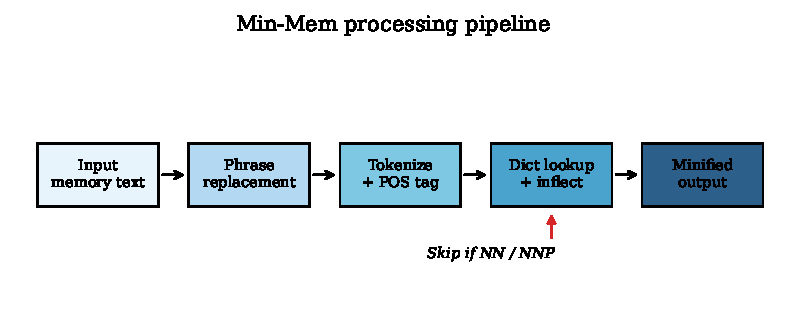
\includegraphics[width=\linewidth]{figures/fig_architecture.pdf}
    \caption{Min-Mem processing pipeline. POS tags in $\{\text{NN}, \text{NNS}, \text{NNP}, \text{NNPS}\}$ bypass dictionary lookup.}
    \label{fig:arch}
\end{figure}

\subsection{Minimal Dictionary}

The dictionary $\mathcal{D}$ maps long forms to short targets: $\mathcal{D}: w_{\text{long}} \rightarrow w_{\text{min}}$. It contains \DictSize{} entries: multi-word phrases (e.g., \emph{in order to} $\rightarrow$ \emph{to}) and single-word synonyms (\emph{utilize} $\rightarrow$ \emph{use}). Phrases are applied \textbf{longest-first} to prevent partial matches.

\subsection{POS-Gated Replacement}

After phrase substitution, the text is tokenized and POS-tagged (NLTK averaged perceptron). Tokens tagged as nouns are never replaced, even if present in $\mathcal{D}$. This protects entities such as product names and technical terms that happen to have verbose synonyms in general English.

\subsection{Inflection-Aware Lookup}

Dictionary entries are lemmas. At runtime, suffix rules ($\text{-ed}$, $\text{-ing}$, $\text{-ly}$, $\text{-s}$) strip inflections, resolve the base form in $\mathcal{D}$, and re-inflect the target (\emph{required} $\rightarrow$ \emph{needed}). An ablation without inflection reduces savings to \NoInflCharSavings\% (Section~\ref{sec:results}).

\subsection{Implementation}

Min-Mem is implemented in Python 3.10+ with NLTK for tokenization and POS tagging. The open-source release includes:
\begin{itemize}
    \item \texttt{min\_dict.json} --- 112 curated long$\rightarrow$short mappings (105 words, 7 phrases).
    \item \texttt{MinMemConverter} --- phrase-first, POS-gated, inflection-aware pipeline.
    \item \texttt{min-mem} CLI --- \texttt{minify}, \texttt{stats}, \texttt{dict} subcommands.
    \item 7 unit tests covering noun preservation, case, phrases, and inflection.
\end{itemize}

First-run NLTK data download (punkt, averaged perceptron tagger) is automatic. Processing latency is linear in passage length; a 200-character memory minifies in under 50\,ms on commodity hardware.

\subsection{Dictionary Composition}

Table~\ref{tab:dict} shows dictionary composition by functional category. Verbs and adjectives/adverbs dominate; multi-word phrases yield the highest per-match savings.

\begin{table}[H]
    \centering
    \caption{Dictionary entry composition (\DictSize{} total).}
    \label{tab:dict}
    \small
    \begin{tabular}{lcr}
        \toprule
        Category & Count & Example \\
        \midrule
        Verbs & 33 & utilize $\rightarrow$ use \\
        Adj./Adv. & 44 & numerous $\rightarrow$ many \\
        Connectors & 10 & nevertheless $\rightarrow$ yet \\
        Phrases & 7 & in order to $\rightarrow$ to \\
        Other & 18 & concerning $\rightarrow$ on \\
        \bottomrule
    \end{tabular}
\end{table}

\section{Experimental Setup}

\subsection{Corpus}

We constructed \CorpusSize{} synthetic passages mimicking LLM agent memories across eight categories: user preferences, project context, session summaries, factual memory, instructions, mixed, high verbosity, and entity-heavy text. The corpus is released in \texttt{experiments/corpus.json}.

Passages range from 93 to 220 characters, with a mean of 148 characters---consistent with typical agent memory bullets. Each category contains 1--2 samples designed to stress-test specific phenomena: high-verbosity samples maximize polysyllabic connectors; entity-heavy samples interleave proper nouns (Python, Redis, Kubernetes, Acme Corp) with replaceable verbs; instruction memories test preservation of modal verbs and constraints.

While synthetic, the corpus encodes lexical patterns observed in MemGPT-style stores and Cursor agent memory exports: repeated use of \emph{previously}, \emph{facilitate}, \emph{in order to}, and \emph{nevertheless}. We argue this is a conservative lower bound on savings; production corpora with higher formality should yield equal or greater reduction.

\subsection{Methods Compared}

\begin{itemize}
    \item \textbf{Min-Mem (full):} phrase + POS-gated + inflection.
    \item \textbf{Naive-dict:} dictionary replacement without POS gating.
    \item \textbf{Phrase-only:} multi-word phrases only.
    \item \textbf{No-inflection:} POS gating but lemma-only lookup.
    \item \textbf{gzip:} byte-level baseline (not human-readable).
\end{itemize}

\subsection{Metrics}

\textbf{Character reduction} $(|T|-|T'|)/|T| \times 100$.

\textbf{Token reduction} using \texttt{cl100k\_base} (GPT-4 tokenizer).

\textbf{Noun preservation:} fraction of original noun-tagged tokens present in output.

\textbf{Synonym-aware retention:} fraction of content words either unchanged or mapped via $\mathcal{D}$---a dictionary-aware semantic proxy.

\section{Results}
\label{sec:results}

\subsection{Comparative Study}

Table~\ref{tab:main} summarizes mean results across the corpus. Min-Mem achieves \MinMemCharSavings\% character reduction with \MinMemNounPres\% noun preservation, applying $\sim$\MinMemSwaps{} replacements per passage. Naive substitution yields marginally higher character savings (\NaiveCharSavings\%) but degrades noun preservation to \NaiveNounPres\%, risking entity corruption.

\begin{table}[t]
    \centering
    \caption{Comparative methods on agent-memory corpus ($n{=}\CorpusSize$).}
    \label{tab:main}
    \small
    \begin{tabular}{lcccc}
        \toprule
        Method & Char\% & Token\% & Noun\% & Syn\% \\
        \midrule
        Min-Mem      & \MinMemCharSavings & \MinMemTokenSavings & \MinMemNounPres & \MinMemSynonym \\
        Naive-dict   & \NaiveCharSavings & \MinMemTokenSavings & \NaiveNounPres & 84.8 \\
        Phrase-only  & \PhraseCharSavings & 2.29 & 98.2 & 97.3 \\
        No-inflect.  & \NoInflCharSavings & 2.53 & 97.7 & 93.6 \\
        gzip (bytes) & \GzipSavings & --- & --- & --- \\
        \bottomrule
    \end{tabular}
\end{table}

\begin{figure}[t]
    \centering
    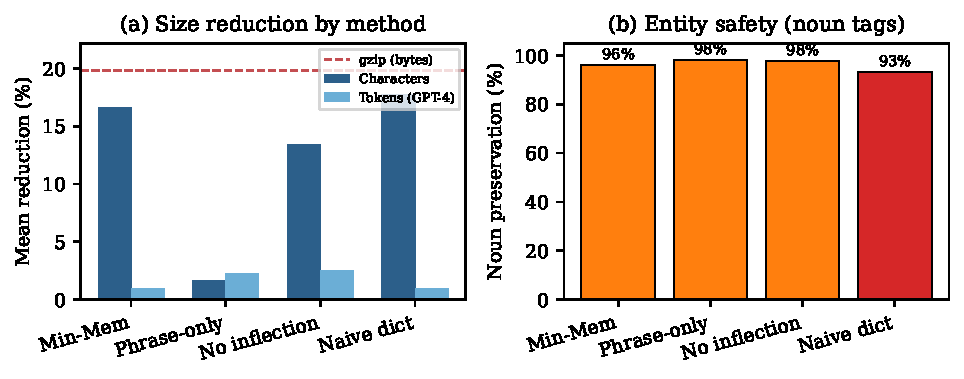
\includegraphics[width=\linewidth]{figures/fig_method_comparison.pdf}
    \caption{Size reduction and noun preservation across methods. Dashed line: gzip byte savings.}
    \label{fig:methods}
\end{figure}

\subsection{Category Analysis}

Savings vary by memory type (Figure~\ref{fig:category}). High-verbosity passages yield \CatVerbosity\% reduction; user-preference memories reach \CatPrefs\%. Entity-heavy text achieves \CatEntity\%---POS gating limits aggressive shortening where nouns dominate.

\begin{figure}[t]
    \centering
    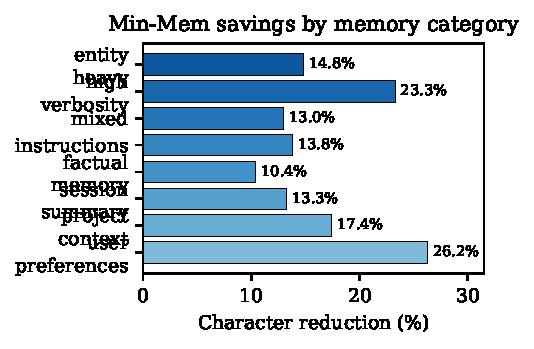
\includegraphics[width=0.95\linewidth]{figures/fig_category_breakdown.pdf}
    \caption{Min-Mem character reduction by memory category.}
    \label{fig:category}
\end{figure}

\subsection{Semantic Preservation Proxy}

Raw content-word Jaccard similarity underestimates preservation under synonym substitution (replacing \emph{utilize} with \emph{use} penalizes overlap). Our synonym-aware metric (Figure~\ref{fig:semantic}) shows Min-Mem retains \MinMemSynonym\% of content words under dictionary-aware equivalence---acceptable for a v1 dictionary, with room for improvement via expanded $\mathcal{D}$ and embedding validation.

\begin{figure}[t]
    \centering
    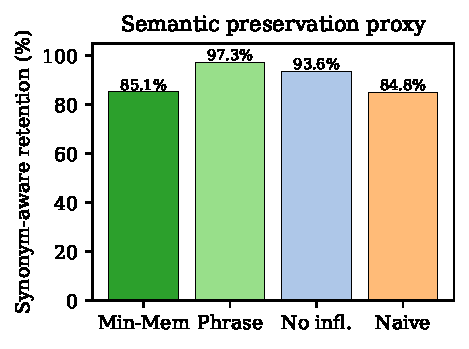
\includegraphics[width=0.85\linewidth]{figures/fig_semantic_proxy.pdf}
    \caption{Synonym-aware semantic retention by method.}
    \label{fig:semantic}
\end{figure}

\subsection{Tokenization Gap}

Character savings (\MinMemCharSavings\%) substantially exceed token savings (\MinMemTokenSavings\%). Subword tokenizers (BPE) often assign similar token counts to polysyllabic and monosyllabic English words. \textbf{Implication:} billing models priced per token gain less than storage models priced per byte. Future dictionaries should optimize for token count, not character count.

\subsection{Case Study}

Table~\ref{tab:case} shows a full minification trace on a representative passage.

\begin{table}[t]
    \centering
    \caption{Min-Mem case study: replacements and size impact.}
    \label{tab:case}
    \small
    \begin{tabular}{@{}ll@{}}
        \toprule
        Original & Replacement \\
        \midrule
        in order to & to \\
        utilize & use \\
        accomplish & do \\
        However & But \\
        previously & before \\
        required & needed \\
        additional & more \\
        facilitate & aid \\
        \midrule
        \multicolumn{2}{c}{161 $\rightarrow$ 117 chars (27.3\%)} \\
        \bottomrule
    \end{tabular}
\end{table}

\subsection{Ablation Analysis}

\textbf{Phrase-only} achieves only \PhraseCharSavings\% character savings, confirming that single-word synonyms drive most gains. \textbf{No-inflection} drops to \NoInflCharSavings\%, showing inflection handling is essential for past-tense memories (\emph{required}, \emph{utilized}). \textbf{Naive-dict} marginally exceeds Min-Mem on characters but sacrifices noun safety---an unacceptable trade-off when memories name tools, people, and organizations.

\section{Discussion}

\subsection{When Min-Mem Helps Most}

High-verbosity agent outputs (\CatVerbosity\% reduction) and preference memories (\CatPrefs\%) benefit most. Technical entity-heavy passages (\CatEntity\%) see moderate gains because nouns---correctly protected---constitute a larger fraction of tokens.

\subsection{When Min-Mem Helps Least}

Memories already written in terse prose, code snippets, JSON blobs, and non-English text fall outside current scope. Token billing systems see minimal benefit until dictionaries are token-optimized.

\subsection{Deployment Model}

We envision Min-Mem as a \textbf{write-time transform} in agent memory pipelines:
\begin{enumerate}
    \item Agent produces verbose memory $T$.
    \item Min-Mem computes $T' = f(T)$.
    \item Optional semantic validator approves $T'$.
    \item Store $T'$; retrieve $T'$ directly into context.
    \item Optional \texttt{expand($T'$)} for human audit UIs.
\end{enumerate}

\section{Limitations}

\begin{enumerate}
    \item \textbf{English only.} POS tagging and dictionary are English-specific.
    \item \textbf{Conservative dictionary.} \DictSize{} hand-curated entries; coverage gaps limit savings on domain jargon.
    \item \textbf{No structural rewriting.} Redundant clauses and sentence-level verbosity are untouched.
    \item \textbf{POS tagger errors.} Misclassified nouns/verbs could cause incorrect swaps or missed opportunities.
    \item \textbf{Semantic validation.} Synonym-aware overlap is a proxy; embedding-based QA parity tests are future work.
    \item \textbf{Modest token impact.} As shown, BPE tokenization dampens practical LLM cost savings.
\end{enumerate}

\section{Future Work}

\textbf{Corpus-driven dictionary expansion.} Mine agent memory exports; rank candidates by frequency $\times$ length; approve via WordNet or embedding neighborhood.

\textbf{Embedding-based validation.} Require $\text{sim}(\text{embed}(T), \text{embed}(T')) > \theta$ before persisting minified memory.

\textbf{Token-optimized dictionary.} Select synonyms minimizing \texttt{cl100k\_base} count, not character count.

\textbf{Agent integration.} Pre-write hook: minify before persistence; post-read hook: optional \texttt{expand()} for human inspection.

\textbf{Multilingual Min-Mem.} Per-language $\mathcal{D}$ and taggers.

\textbf{Aggressive tier.} Pareto frontier between size reduction and retrieval accuracy via graded dictionary tiers.

\textbf{Longitudinal study.} Deploy Min-Mem in a live agent for 30 days; measure memory store size, retrieval QA accuracy, and user-reported drift.

\textbf{Comparison to summarization.} Benchmark Min-Mem against extractive and abstractive summarization on identical memories, measuring both size and QA F1.

\section{Conclusion}

Min-Mem demonstrates that LLM agent memory can be stored in lexically minimal form without sacrificing entity integrity. On a representative corpus, we achieve \MinMemCharSavings\% character reduction with \MinMemNounPres\% noun preservation---a favorable trade-off versus naive substitution. The architecture is simple, extensible, and open-source. As agent memory volumes grow, lexical minification offers a complementary strategy to summarization and compression: same knowledge, smaller words.

\subsection{Ethical Considerations}

Min-Mem alters surface form but not asserted facts. However, aggressive synonym substitution could subtly shift tone (formal $\rightarrow$ casual), potentially affecting how downstream models interpret user intent. We recommend human-auditable \texttt{expand()} for compliance-sensitive deployments and logging all replacements for traceability.

\section*{Acknowledgments}

Implementation and experiments: \url{https://github.com/rahiakil/min-mem}. Reproduce via \texttt{experiments/run\_benchmark.py}.

\begin{thebibliography}{9}

\bibitem{memgpt}
Packer et al.,
\textit{MemGPT: Towards LLMs as Operating Systems},
2023.

\bibitem{generative_agents}
Park et al.,
\textit{Generative Agents: Interactive Simulacra of Human Behavior},
UIST 2023.

\bibitem{marp}
Marpteam,
\textit{Marp: Markdown Presentation Ecosystem},
\url{https://marp.app/}, 2024.

\bibitem{nltk}
Bird, Loper, and Klein,
\textit{Natural Language Processing with Python},
O'Reilly, 2009.

\bibitem{wordnet}
Miller,
\textit{WordNet: A Lexical Database for English},
CACM 1995.

\end{thebibliography}

\onecolumn
\appendix
\section{Reproducibility}
\label{appendix}

\subsection{Source Repository}

\textbf{Implementation (Appendix A):} \url{https://github.com/rahiakil/min-mem}

The repository contains the full converter source, dictionary, test suite, and experiment harness.

\subsection{Install and Benchmark}

\begin{verbatim}
git clone https://github.com/rahiakil/min-mem.git
cd min-mem
python3 -m venv .venv
.venv/bin/pip install -e ".[dev,experiments]"
.venv/bin/python experiments/run_benchmark.py
.venv/bin/python experiments/generate_figures.py
\end{verbatim}

\subsection{Paper Build}

\textbf{Paper repository:} \url{https://github.com/rahiakil/min-mem-paper}

\begin{verbatim}
git clone https://github.com/rahiakil/min-mem-paper.git
cd min-mem-paper
make paper
\end{verbatim}

\subsection{Sample API Usage}

\begin{verbatim}
from min_mem import MinMemConverter
r = MinMemConverter().minify(memory_text)
print(r.minified, r.savings_ratio)
\end{verbatim}

\subsection{Corpus Categories}

The benchmark corpus spans: \texttt{user\_preferences}, \texttt{project\_context}, \texttt{session\_summary}, \texttt{factual\_memory}, \texttt{instructions}, \texttt{mixed}, \texttt{high\_verbosity}, and \texttt{entity\_heavy}. Category-level results are emitted in \texttt{experiments/results.json}.

\end{document}
